% Figure 2 composite (vector). Build: lualatex fig2_assemble.tex
% Page 183 x 170 mm (<= 183 mm wide; height reduced from the previous 174 mm).
% Every panel is drawn at its final placement size, so each is placed at scale
% 1.00 and on-page type stays 5.2-7 pt. Panel PDFs carry a 0.01 in savefig pad,
% hence the .51 mm widths below.
%
% Grid contract:
%   * content column runs x = 6 mm to 179.51 mm in every row (equal margins)
%   * row gutters are 5.49 mm (rows 1-2) and 5.49 mm (rows 2-3); column gutters
%     are 5.49 mm in row 1 and 5.99 mm in rows 2 and 3
%   * panels within a row share one top edge and one baseline (identical heights)
%   * b and c additionally share one axes band, so their 20 rows line up; the
%     method-label column and the feature-space key are drawn once, inside b
\documentclass[tikz,border=0mm]{standalone}
\usepackage{graphicx}
% Shared font contract for every AllelePerturb composite (Nature Methods).
% Input from each figN_assemble.tex as % Shared font contract for every AllelePerturb composite (Nature Methods).
% Input from each figN_assemble.tex as % Shared font contract for every AllelePerturb composite (Nature Methods).
% Input from each figN_assemble.tex as \input{../nm_fonts.tex}.
%
% ONE sans family per figure. The matplotlib panels resolve their family through
% nm_style.py as Arial -> Helvetica -> Liberation Sans (first installed wins), so
% the panel letters stamped by figN_assemble.tex must resolve the same way or the
% composite embeds two families. Until 2026-07-31 these files loaded helvet, which
% put NimbusSanL (a Helvetica clone, Type 1) in every composite for the letters
% while every other glyph was Liberation Sans (an Arial clone, CID TrueType).
% Nature Methods asks for Arial or Helvetica; it does not accept both in one figure.
%
% Requires lualatex, i.e. fontspec + luaotfload (Debian/Ubuntu: texlive-luatex).
% Build every composite with:
%     lualatex -interaction=nonstopmode figN_assemble.tex
% pdflatex will fail here by design: it cannot load a system OpenType/TrueType
% family, and silently falling back to helvet is the defect this file removes.
\usepackage{fontspec}
\IfFontExistsTF{Arial}%
  {\setsansfont{Arial}}%
  {\IfFontExistsTF{Helvetica}%
     {\setsansfont{Helvetica}}%
     {\setsansfont{Liberation Sans}}}
\renewcommand{\familydefault}{\sfdefault}
.
%
% ONE sans family per figure. The matplotlib panels resolve their family through
% nm_style.py as Arial -> Helvetica -> Liberation Sans (first installed wins), so
% the panel letters stamped by figN_assemble.tex must resolve the same way or the
% composite embeds two families. Until 2026-07-31 these files loaded helvet, which
% put NimbusSanL (a Helvetica clone, Type 1) in every composite for the letters
% while every other glyph was Liberation Sans (an Arial clone, CID TrueType).
% Nature Methods asks for Arial or Helvetica; it does not accept both in one figure.
%
% Requires lualatex, i.e. fontspec + luaotfload (Debian/Ubuntu: texlive-luatex).
% Build every composite with:
%     lualatex -interaction=nonstopmode figN_assemble.tex
% pdflatex will fail here by design: it cannot load a system OpenType/TrueType
% family, and silently falling back to helvet is the defect this file removes.
\usepackage{fontspec}
\IfFontExistsTF{Arial}%
  {\setsansfont{Arial}}%
  {\IfFontExistsTF{Helvetica}%
     {\setsansfont{Helvetica}}%
     {\setsansfont{Liberation Sans}}}
\renewcommand{\familydefault}{\sfdefault}
.
%
% ONE sans family per figure. The matplotlib panels resolve their family through
% nm_style.py as Arial -> Helvetica -> Liberation Sans (first installed wins), so
% the panel letters stamped by figN_assemble.tex must resolve the same way or the
% composite embeds two families. Until 2026-07-31 these files loaded helvet, which
% put NimbusSanL (a Helvetica clone, Type 1) in every composite for the letters
% while every other glyph was Liberation Sans (an Arial clone, CID TrueType).
% Nature Methods asks for Arial or Helvetica; it does not accept both in one figure.
%
% Requires lualatex, i.e. fontspec + luaotfload (Debian/Ubuntu: texlive-luatex).
% Build every composite with:
%     lualatex -interaction=nonstopmode figN_assemble.tex
% pdflatex will fail here by design: it cannot load a system OpenType/TrueType
% family, and silently falling back to helvet is the defect this file removes.
\usepackage{fontspec}
\IfFontExistsTF{Arial}%
  {\setsansfont{Arial}}%
  {\IfFontExistsTF{Helvetica}%
     {\setsansfont{Helvetica}}%
     {\setsansfont{Liberation Sans}}}
\renewcommand{\familydefault}{\sfdefault}

\begin{document}
\begin{tikzpicture}[x=1mm,y=1mm]
  \useasboundingbox (0,0) rectangle (183,170);
  % ---- row 1 (h 63.51): a schematic | b PDS forest | c Pearson forest -------
  \node[anchor=north west,inner sep=0] at (6,166.5)   {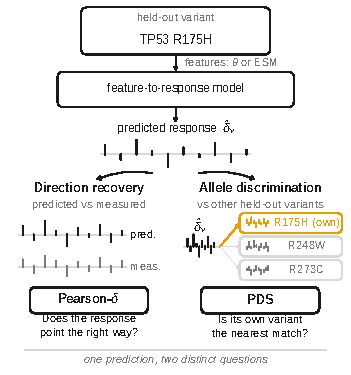
\includegraphics[width=59.51mm]{fig2a_evaluation.pdf}};
  \node[anchor=north west,inner sep=0] at (71,166.5)  {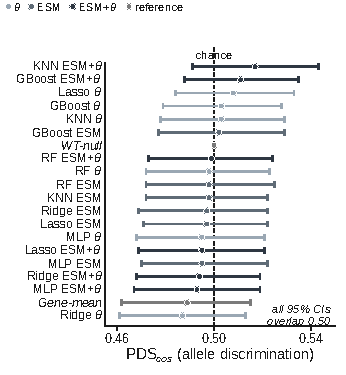
\includegraphics[width=58.51mm]{fig2b_pds_forest.pdf}};
  \node[anchor=north west,inner sep=0] at (135,166.5) {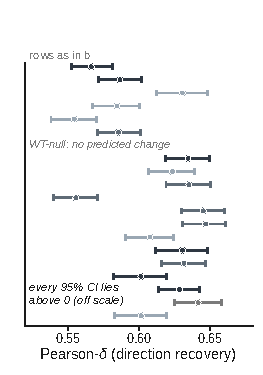
\includegraphics[width=44.51mm]{fig2c_pearson_forest.pdf}};
  % ---- row 2 (h 44.51): d PDS-vs-Pearson scatter | e DE fidelity gradient ---
  \node[anchor=north west,inner sep=0] at (6,97.5)    {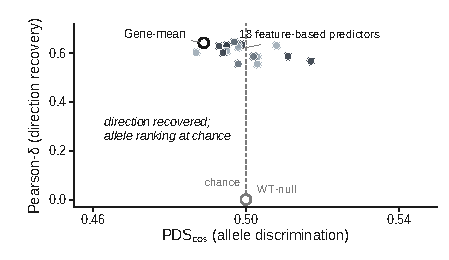
\includegraphics[width=76.51mm]{fig2d_scatter.pdf}};
  \node[anchor=north west,inner sep=0] at (88.5,97.5) {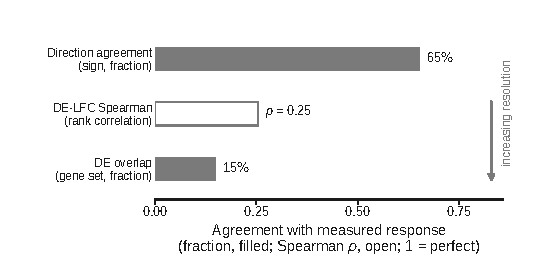
\includegraphics[width=91.01mm]{fig2e_de_gradient.pdf}};
  % ---- row 3 (h 44.51): f per-gene gap | g representative TP53 variants -----
  \node[anchor=north west,inner sep=0] at (6,47.5)    {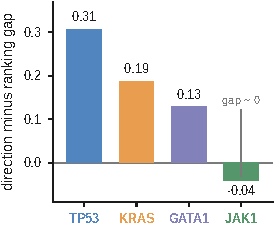
\includegraphics[width=46.51mm]{fig2f_gene_gap.pdf}};
  \node[anchor=north west,inner sep=0] at (58.5,47.5) {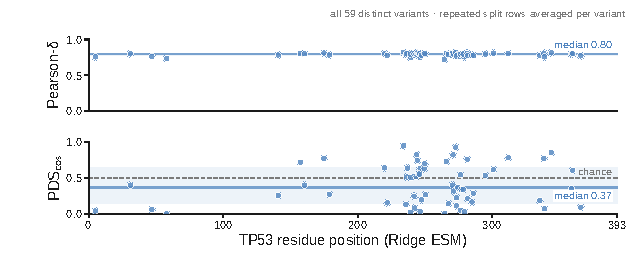
\includegraphics[width=121.01mm]{fig2g_pervariant.pdf}};
  % ---- panel letters: lowercase bold, 8 pt at final size --------------------
  \tikzset{plab/.style={font=\fontsize{8}{9}\selectfont\bfseries,anchor=north west,inner sep=0}}
  \node[plab] at (1.5,168) {a};  \node[plab] at (66.5,168) {b}; \node[plab] at (130.5,168) {c};
  \node[plab] at (1.5,99)  {d};  \node[plab] at (84,99)    {e};
  \node[plab] at (1.5,49)  {f};  \node[plab] at (54,49)    {g};
\end{tikzpicture}
\end{document}
